%
% fig-kubisch.tex
%
% (c) 2025 Prof Dr Andreas Müller
%
\begin{figure}
\centering
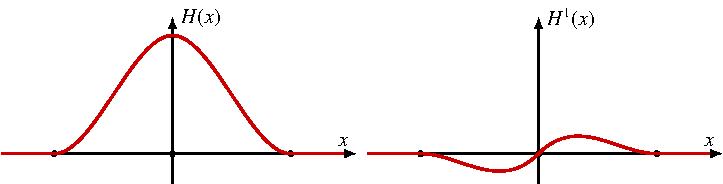
\includegraphics{chapters/090-pdenumerik/images/kubisch.pdf}
\caption{Kubische Approximationsfunktionen für die Methode der
finiten Elemente in einer Dimension.
Für ganzzahlige Argumente (schwarze Punkte auf der $x$-Achse)
hat die Funktion $H(x)$ nur bei $x=0$ den Wert $1$, alle anderen
Funktionswerte und alle Ableitungen verschwinden.
Die Funktion $H^1(x)$ ist in allen Gitterpunkten ebenso wie
ihre Ableitung $=0$ mit Ausnahme des Punktes $x=0$, wo die
Ableitung $=1$ ist.
\label{buch:pdenumerik:fem:fig:kubisch}}
\end{figure}
